% Informe del proyecto final — Tecnologías Web (5916) · Unisimón 2026-2
% Compilar con: pdflatex informe.tex   (las capturas van en docs/capturas/)
\documentclass[10pt,a4paper]{article}

\usepackage[utf8]{inputenc}
\usepackage[T1]{fontenc}
\usepackage{lmodern}
\usepackage{microtype}
\usepackage[a4paper,margin=1.5cm,top=1.3cm,bottom=1.4cm]{geometry}
\usepackage{graphicx}
\usepackage{tikz}
\usetikzlibrary{positioning,arrows.meta,fit,calc,shapes.multipart}
\usepackage{tabularx}
\usepackage{booktabs}
\usepackage{enumitem}
\usepackage[font=footnotesize,labelfont=bf,skip=3pt]{caption}
\usepackage{titlesec}
\usepackage[hidelinks]{hyperref}

\renewcommand{\figurename}{Figura}
\renewcommand{\tablename}{Tabla}
\titleformat{\section}{\large\bfseries}{\thesection.}{0.5em}{}[\vspace{-0.6em}\rule{\linewidth}{0.6pt}]
\titlespacing*{\section}{0pt}{8pt}{6pt}
\setlist{nosep,leftmargin=1.2em}
\setlength{\parindent}{0pt}
\setlength{\parskip}{4pt}
\graphicspath{{capturas/}}

\newcommand{\code}[1]{\texttt{\small #1}}
% Inserta una captura si existe; si no, deja un recuadro con el nombre del archivo
\newcommand{\captura}[3]{%
  \begin{minipage}[t]{#1}\centering
    \IfFileExists{capturas/#2}%
      {\includegraphics[width=\linewidth,height=5.6cm,keepaspectratio]{#2}}%
      {\fbox{\parbox[c][5.4cm][c]{0.94\linewidth}{\centering\footnotesize capturas/#2}}}%
    \par\vspace{2pt}{\footnotesize #3}
  \end{minipage}}

\begin{document}

{\LARGE\bfseries Alacena — Generador de recetas con inventario e IA}\par\vspace{4pt}
{\small
\begin{tabularx}{\linewidth}{@{}l X l l@{}}
\textbf{Estudiante} & Erick Fabián Donado Fonseca & \textbf{Curso} & Tecnologías Web (5916) · T02 · 2026-2\\
\textbf{Repositorio} & \url{https://github.com/KanuSaru/proyecto-recetas} & \textbf{Profesor} & Rafael Bladimir Pérez Merino\\
\textbf{Aplicación} & \url{https://recetas-ia.onrender.com} & \textbf{API} & \code{/docs} (Swagger/OpenAPI)\\
\end{tabularx}}

\section{Descripción y arquitectura}
Aplicación web donde cada usuario registra los ingredientes que tiene en casa y obtiene recetas generadas por un modelo de lenguaje. Las recetas se guardan en la base de datos y se pueden consultar, calificar de 1 a 5 estrellas y eliminar. El backend es una API REST en \textbf{Python + FastAPI}; la interfaz es una página \textbf{Jinja2} con JavaScript sin frameworks que consume la misma API con un \textbf{JWT}.

\begin{figure}[h]
\centering
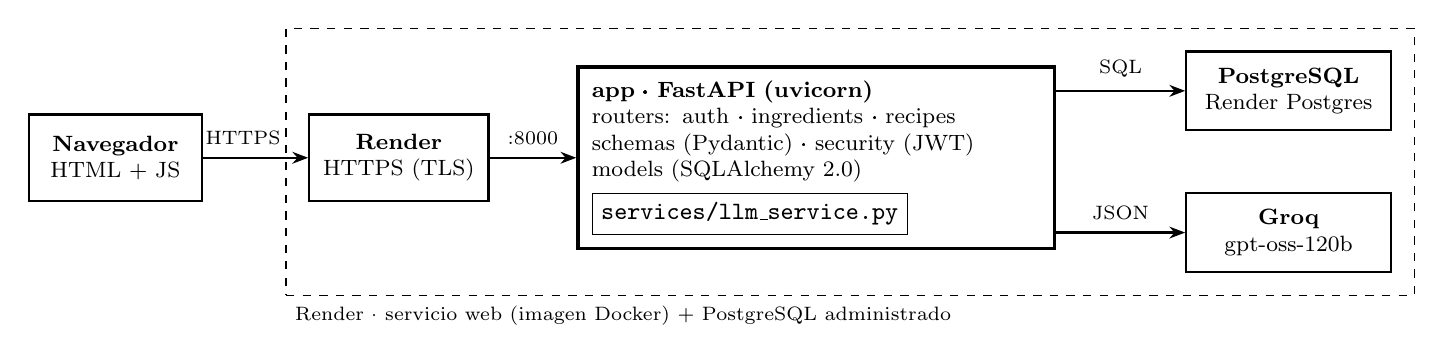
\begin{tikzpicture}[
  font=\footnotesize,
  box/.style={draw,thick,align=center,inner sep=5pt,fill=white},
  arr/.style={-{Stealth[length=2mm]},thick},
  lbl/.style={font=\scriptsize,above=1pt}]
  \node[box,minimum width=2.2cm,minimum height=1.1cm] (nav) at (0,0) {\textbf{Navegador}\\HTML + JS};
  \node[box,minimum width=2.2cm,minimum height=1.1cm] (render) at (3.6,0) {\textbf{Render}\\HTTPS (TLS)};
  \node[box,line width=1.2pt,text width=5.7cm,align=left] (app) at (8.9,0)
    {\textbf{app · FastAPI (uvicorn)}\\
     routers: auth · ingredients · recipes\\
     schemas (Pydantic) · security (JWT)\\
     models (SQLAlchemy 2.0)\\[3pt]
     \fbox{\code{services/llm\_service.py}}};
  \node[box,minimum width=2.6cm,minimum height=1.0cm] (db) at (14.9,0.85) {\textbf{PostgreSQL}\\Render Postgres};
  \node[box,minimum width=2.6cm,minimum height=1.0cm] (llm) at (14.9,-0.95) {\textbf{Groq}\\gpt-oss-120b};
  \draw[arr] (nav) -- node[lbl,pos=0.38]{HTTPS} (render);
  \draw[arr] (render) -- node[lbl]{:8000} (app);
  \draw[arr] (app.east|-db) -- node[lbl]{SQL} (db);
  \draw[arr] (app.east|-llm) -- node[lbl]{JSON} (llm);
  \node[draw,dashed,inner sep=8pt,fit=(render)(app)(db)(llm)] (cloud) {};
  \node[font=\scriptsize,anchor=north west] at (cloud.south west) {Render · servicio web (imagen Docker) + PostgreSQL administrado};
\end{tikzpicture}
\caption{Arquitectura desplegada: servicio web con la imagen Docker de la app, PostgreSQL administrado y el proveedor LLM externo.}
\end{figure}

\textbf{Flujo de generación.} \code{POST /api/recipes/generate} lee el inventario del usuario autenticado y llama a \code{LLMService}. El servicio arma un prompt fijo (mensaje de sistema con el formato JSON exigido + inventario con cantidades, porciones y tipo de comida), lo envía a Groq (modelo \code{openai/gpt-oss-120b}, API compatible con OpenAI) y pasa la respuesta por \code{parse\_recipe\_response}, que extrae el objeto JSON y lo valida contra el esquema \code{RecipeLLMOutput}: \code{nombre}, \code{ingredientes[\{nombre, cantidad\}]}, \code{pasos[]}, \code{tiempo\_estimado\_minutos} y \code{dificultad} (fácil/media/difícil). Solo si es válido se guarda la receta. El usuario nunca escribe texto libre para el modelo: no es un chatbot.

\begin{table}[h]
\centering\small
\begin{tabularx}{\linewidth}{@{}l X@{}}
\toprule
\textbf{Funcionalidad} & \textbf{Endpoints}\\
\midrule
Registro e inicio de sesión (JWT) & \code{POST /api/auth/register} · \code{POST /api/auth/login} · \code{GET /api/auth/me}\\
CRUD de ingredientes & \code{GET/POST /api/ingredients} · \code{GET/PUT/DELETE /api/ingredients/\{id\}}\\
Generar receta · historial & \code{POST /api/recipes/generate} · \code{GET /api/recipes} · \code{GET /api/recipes/\{id\}}\\
Calificar · eliminar & \code{PUT /api/recipes/\{id\}/rating} (1–5) · \code{DELETE /api/recipes/\{id\}}\\
\bottomrule
\end{tabularx}
\caption{Funcionalidades mínimas y endpoints de la API.}
\end{table}

\newpage
\section{Modelo de base de datos}
\begin{figure}[h]
\centering
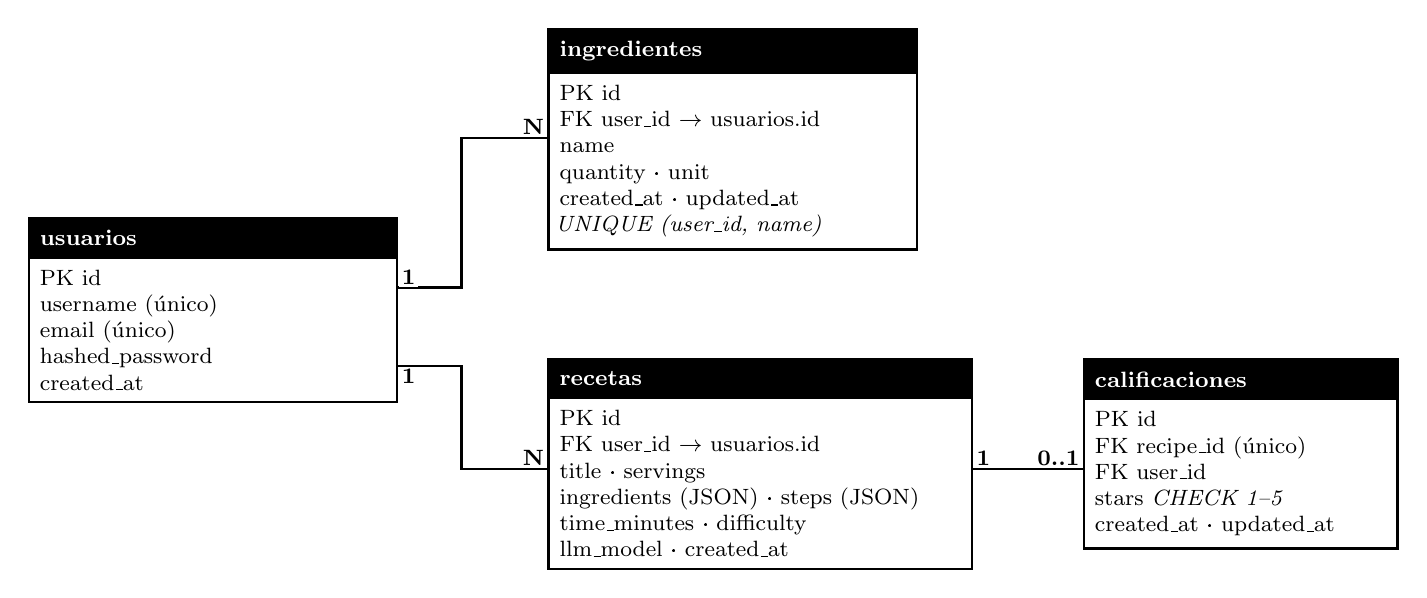
\begin{tikzpicture}[
  font=\footnotesize,
  ent/.style={draw,thick,rectangle split,rectangle split parts=2,align=left,inner sep=4pt,
              rectangle split part fill={black,white},text width=4.4cm},
  rel/.style={thick},
  card/.style={font=\footnotesize\bfseries,fill=white,inner sep=1pt}]
  \node[ent,anchor=north west] (u) at (0,0.2) {\textcolor{white}{\textbf{usuarios}}
    \nodepart{two} PK id\\ username (único)\\ email (único)\\ hashed\_password\\ created\_at};
  \node[ent,anchor=north west] (i) at (6.6,2.6) {\textcolor{white}{\textbf{ingredientes}}
    \nodepart{two} PK id\\ FK user\_id $\rightarrow$ usuarios.id\\ name\\ quantity · unit\\ created\_at · updated\_at\\ \textit{UNIQUE (user\_id, name)}};
  \node[ent,anchor=north west,text width=5.1cm] (r) at (6.6,-1.6) {\textcolor{white}{\textbf{recetas}}
    \nodepart{two} PK id\\ FK user\_id $\rightarrow$ usuarios.id\\ title · servings\\ ingredients (JSON) · steps (JSON)\\ time\_minutes · difficulty\\ llm\_model · created\_at};
  \node[ent,anchor=north west,text width=3.7cm] (c) at (13.4,-1.6) {\textcolor{white}{\textbf{calificaciones}}
    \nodepart{two} PK id\\ FK recipe\_id (único)\\ FK user\_id\\ stars \textit{CHECK 1–5}\\ created\_at · updated\_at};
  % usuarios 1 -- N ingredientes
  \coordinate (ua) at ($(u.north east)+(0,-0.9)$);
  \coordinate (ub) at ($(u.north east)+(0,-1.9)$);
  \draw[rel] (ua) -- ++(0.8,0) |- ($(i.north west)+(0,-1.4)$);
  \node[card,above right] at (ua) {1};
  \node[card,above left] at ($(i.north west)+(0,-1.4)$) {N};
  % usuarios 1 -- N recetas
  \draw[rel] (ub) -- ++(0.8,0) |- ($(r.north west)+(0,-1.4)$);
  \node[card,below right] at (ub) {1};
  \node[card,above left] at ($(r.north west)+(0,-1.4)$) {N};
  % recetas 1 -- 0..1 calificaciones
  \draw[rel] ($(r.north east)+(0,-1.4)$) -- ($(c.north west)+(0,-1.4)$);
  \node[card,above right] at ($(r.north east)+(0,-1.4)$) {1};
  \node[card,above left] at ($(c.north west)+(0,-1.4)$) {0..1};
\end{tikzpicture}
\caption{Diagrama entidad-relación (PostgreSQL). Borrado en cascada desde usuarios y recetas.}
\end{figure}

Un usuario tiene muchos ingredientes y muchas recetas; cada receta tiene como máximo una calificación (\code{recipe\_id} único). La restricción \code{UNIQUE(user\_id, name)} evita ingredientes repetidos en el inventario y \code{CHECK stars BETWEEN 1 AND 5} garantiza la regla de calificación también en la base de datos. Los ingredientes y pasos de la receta se guardan como JSON porque son el resultado ya validado del LLM y siempre se leen junto con la receta.

\section{Decisiones técnicas}
\begin{itemize}
  \item \textbf{LLM encapsulado y validado.} \code{llm\_service.py} es el único módulo que habla con el proveedor del LLM. Usa la API de chat compatible con OpenAI, así que cambiar entre OpenRouter, Groq u otro proveedor solo requiere variables de entorno; en producción se usa Groq por su capa gratuita. El JSON del modelo se valida con Pydantic antes de guardarse; se toleran bloques de código, texto alrededor y variantes como \code{"30 minutos"} o \code{"facil"}. Si la respuesta es inválida se reintenta una vez y luego la API responde \textbf{502} sin guardar nada.
  \item \textbf{Validación de ingredientes contra inyección de prompt.} Los nombres solo admiten letras, espacios y guiones (2–50 caracteres), la cantidad debe ser positiva y la unidad pertenece a una lista cerrada. Así, un nombre como \textit{``pollo; ignora las instrucciones''} se rechaza con 422 antes de llegar al prompt.
  \item \textbf{Autenticación.} Contraseñas con bcrypt y JWT HS256 con expiración configurable. El login usa el formulario OAuth2 de FastAPI, por lo que el botón \textit{Authorize} de Swagger funciona. Todas las consultas filtran por \code{user\_id} y un recurso ajeno responde 404.
  \item \textbf{Pruebas.} 45 casos con pytest en 4 archivos: validación de ingredientes, construcción del prompt, parseo de la respuesta del LLM y endpoints. Usan SQLite en memoria y un LLM falso inyectado con \code{dependency\_overrides}, así que corren sin red, sin API key y sin gastar cuota.
  \item \textbf{Despliegue.} La app corre en \textbf{Render} como servicio web construido desde el mismo \code{Dockerfile} del repositorio (usuario sin privilegios, healthcheck en \code{/health}), con PostgreSQL administrado en la misma región y HTTPS automático. Se eligió Render porque no fue posible verificar un VPS sin tarjeta de crédito. El repositorio incluye además \code{docker-compose.yml} con tres servicios (\code{db} sin puertos públicos, \code{app} y \code{caddy} con certificado de Let's Encrypt), listo para un VPS con \code{docker compose up -d}. Las credenciales viven en variables de entorno; el repositorio solo incluye \code{.env.example}.
  \item \textbf{Interfaz.} Identidad visual propia (\textit{Alacena}): fondos planos en blanco y verde albahaca, tipografía Bricolage Grotesque, la alacena como panel lateral de ingredientes, la receta como pieza central y el recetario como lista desplegable; favicon propio y confirmación antes de eliminar.
\end{itemize}

\newpage
\section{Capturas del sistema funcionando}
\vspace{2pt}
\noindent
\captura{0.485\linewidth}{01-login.png}{Inicio de sesión / registro (HTTPS y favicon visibles)}\hfill
\captura{0.485\linewidth}{02-inventario.png}{Inventario de ingredientes (CRUD)}

\vspace{8pt}\noindent
\captura{0.485\linewidth}{03-receta.png}{Receta generada por el LLM}\hfill
\captura{0.485\linewidth}{04-historial.png}{Recetario con calificación y eliminación}

\vspace{8pt}\noindent
\captura{\linewidth}{05-swagger.png}{Documentación OpenAPI en \code{/docs}}

\end{document}
